\chapter{Performance and User Experience}
\label{chap:perfux}

\section{Performance}

\subsection{Generation performance}
\paragraph{Single folder} - all files are located within same folder \ref{fig:gs}.
\begin{itemize}
	\item \textbf{Add} - on every iteration of measurement were added 10 xlsx files. Thus previously added xlsx files were skipped for js files creation. All js files were skipped. 10 xlsx files read and 10 js generated;
	\item \textbf{New} - all files are newly added on every measurement iteration and number of generated js files is equivalent
\end{itemize}


\begin{figure}[ht]
	\label{fig:gs}
	\centering
	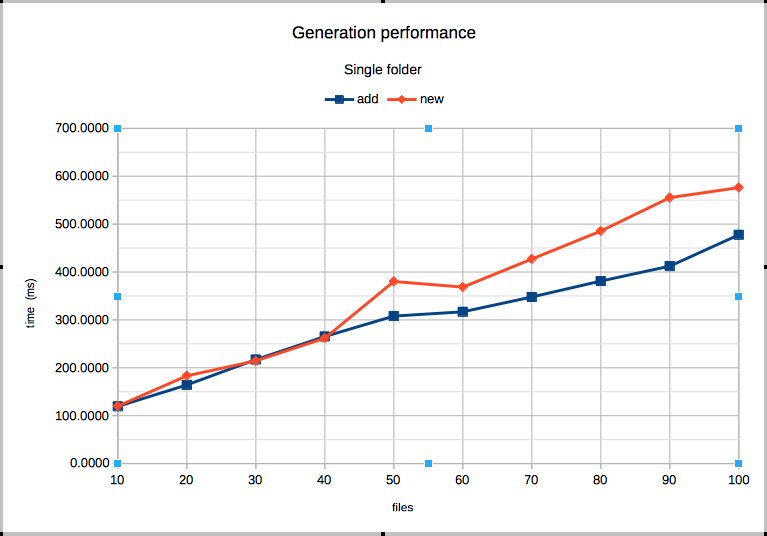
\includegraphics[width=\textwidth]{grafiken/generation_single}
	\caption{Generation performance for files within single folder}
\end{figure}

\paragraph{Nested folder} - all files are located within same folder \ref{fig:gs}.
\begin{itemize}
	\item \textbf{Add} - on every iteration of measurement were added 10 xlsx files in to the folder nested within the folder created inside the folder from the previous iteration. Thus previously added xlsx files were skipped for js files creation. All js files were skipped. 10 xlsx files read and 10 js generated;
	\item \textbf{New} - all files are newly added 10 in folder plus one folder for the same repetative stuff on every measurement iteration and number of generated js files is equivalent
\end{itemize}


\begin{figure}[ht]
	\label{fig:gn}
	\centering
	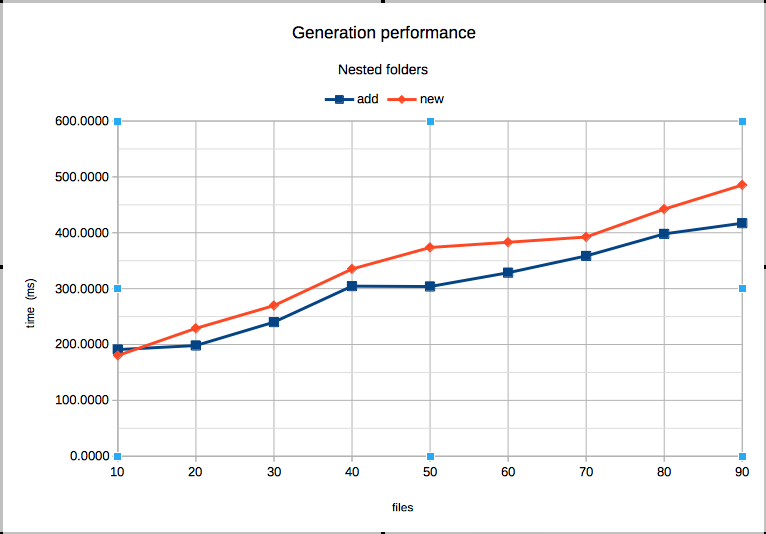
\includegraphics[width=\textwidth]{grafiken/generation_nested}
	\caption{Generation performance for files within nested folders}
\end{figure}

\subsection{Executions performance}

\paragraph{Independent test steps} - all test steps are independent from each other and their call is donde within the same iteration of an event loop\ref{fig:gs}.
\begin{itemize}
	\item \textbf{Scheme comparison} - expected result
	\item \textbf{Deep comparison} - all files are newly added on every measurement iteration and number of generated js files is equivalent
\end{itemize}
\begin{figure}[ht]
	\label{fig:ei}
	\centering
	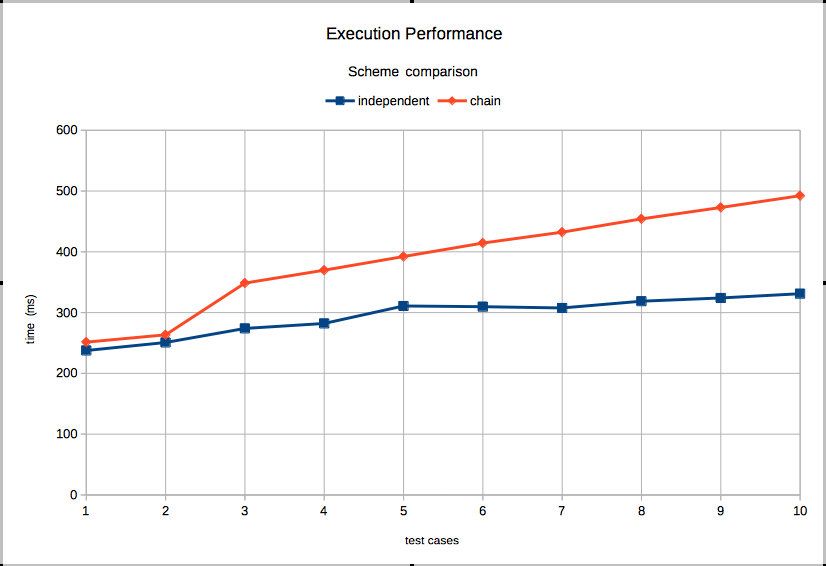
\includegraphics[width=\textwidth]{grafiken/exec_scheme}
	\caption{Execution performance for independent test steps}
\end{figure}

\paragraph{Chain relationship} - all files are located within same folder \ref{fig:gs}.
\begin{itemize}
	\item \textbf{Scheme comparison} - on every iteration of measurement were added 10 xlsx files. Thus previously added xlsx files were skipped for js files creation. All js files were skipped. 10 xlsx files read and 10 js generated;
	\item \textbf{Deep comparison} - all files are newly added on every measurement iteration and number of generated js files is equivalent
\end{itemize}

\begin{figure}[ht]
	\label{fig:ef}
	\centering
	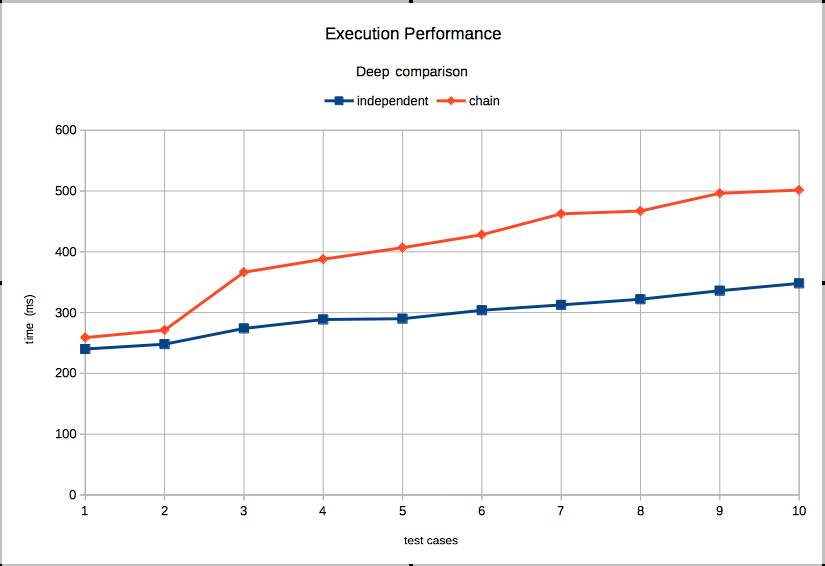
\includegraphics[width=\textwidth]{grafiken/exec_deep}
	\caption{Execution performance for interdependent test steps}
\end{figure}

\section{User Experience}
\subsection{After Scenario Questionnaire}
The ASQ, developed by (Lewis, 1995), is to be given to a study subject after he/she has completed a normal condition scenario. The user is to circle their answers using the provided 7 point scale (the lower the selected score, the higher the subject’s usability satisfaction with their system). After the user has completed the ASQ, the ASQ score can be calculated by taking the average (arithmetic mean) of the 3 questions. If a question is skipped by the subject, the ASQ can be calculated by averaging the remaining scores.
\begin{table}[h]
	\begin{center}
		\begin{tabular}{| l | l | l | l |}
			\hline
			\textbf{Property} & \textbf{Satisfaction 1 }  & \textbf{Satisfaction 4 } & \textbf{Satisfaction 6 }\\
			\hline
			The ease of completing this task. & 1-7  & 1-7 & 1-7 \\
			\hline
			The amount of time it took to complete this task & 1-7 & 1-7 & 1-7 \\
			\hline
			The support information  & 1-7 & 1-7 & 1-7 \\
			\hline
		\end{tabular}
	\end{center}
	\caption{After Scenario Questionnaire}
\end{table}

\subsection{Post Study System Usability Questionnaire}
The PSSUQ is provided to the subject after they have completed all normal condition scenarios. Like the ASQ, the PSSUQ requires that the user circle their response to each question based on a 7-point scale (where the lower the response, the higher the subject’s usability satisfaction with their system). The subject can also clarify their answers on the PSSUQ by adding comments in the provided spaces.
After the subject has completed filling out the PSSUQ, it is good practice for the analyst to quickly go over the subject’s answers in order to make sure the subject hasn’t missed anything and that all comments are understood.
The list of questions:
\begin{itemize}
	\item Overall, I am satisfied with how easy it is to use this system.
	\item It was simple to use this system.
	\item I could effectively complete the tasks and scenarios using this system.
	\item I was able to complete the tasks and scenarios quickly using this system.
	\item I was able to efficiently complete the tasks and scenarios using this system.
	\item I felt comfortable using this system.
	\item It was easy to learn to use this system.
	\item I believe I could become productive quickly using this system.
	\item The system gave error messages that clearly told me how to fix problems.
	\item Whenever I made a mistake using the system, I could recover easily and quickly.
	\item The information (such as on-line help, on-screen messages and other documentation) provided with this system was clear.
	\item It was easy to find the information I needed.
	\item The information provided for the system was easy to understand.
	\item The information was effective in helping me complete the tasks and scenarios.
	\item The organization of information on the system screens was clear.
	\item The interface of this system was pleasant.
	\item I liked using the interface of this system.
	\item This system has all the functions and capabilities I expect it to have.
	\item Overall, I am satisfied with this system.
\end{itemize}
%
%\begin{table}[h]
%	\begin{center}
%		\begin{tabular}{| l | l | }
%			\hline
%			\textbf{Property} & \textbf{Satisfaction} \\
%			\hline
%			Overall, I am satisfied with how easy it is to use this system. & 512  \\
%			\hline
%			It was simple to use this system. & 512  \\
%			\hline
%			I could effectively complete the tasks and scenarios using this system. & 512  \\
%			\hline
%			I was able to complete the tasks and scenarios quickly using this system. & 512  \\
%			\hline
%			I was able to efficiently complete the tasks and scenarios using this system. & 512  \\
%			\hline
%			I felt comfortable using this system. & 512  \\
%			\hline
%			It was easy to learn to use this system. & 512  \\
%			\hline
%			I believe I could become productive quickly using this system. & 512  \\
%			\hline
%			The system gave error messages that clearly told me how to fix problems. & 512  \\
%			\hline
%			Whenever I made a mistake using the system, I could recover easily and quickly. & 512  \\
%			\hline
%			The information (such as on-line help, on-screen messages and other documentation) provided with this system was clear. & 512  \\
%			\hline
%			It was easy to find the information I needed. & 512  \\
%			\hline
%			The information provided for the system was easy to understand. & 512  \\
%			\hline
%			The information was effective in helping me complete the tasks and scenarios. & 512  \\
%			\hline
%			The organization of information on the system screens was clear. & 512  \\
%			\hline
%			 The interface of this system was pleasant. & 512  \\
%			\hline
%			I liked using the interface of this system. & 512  \\
%			\hline
%			This system has all the functions and capabilities I expect it to have. & 512  \\
%			\hline
%			Overall, I am satisfied with this system. & 512  \\
%			\hline
%		\end{tabular}
%	\end{center}
%	\caption{Post Study System Usability Questionnaire}
%\end{table}

The PSSUQ can be used to produce the following measures:
\begin{itemize}
	\item OVERALL – Overall user satisfaction with their system – calculated by taking the average of questions 1-19
	\item SYSUSE – System usefulness – calculated by taking the average of questions 1-8
	\item INFOQUAL – Information quality – calculated by taking the average of questions 9-15
	\item INTERQUAL – Interface quality – calculated by taking the average of questions 16-18
\end{itemize}
\begin{table}[h]
	\begin{center}
		\begin{tabular}{| l | l | l | }
			\hline
			\textbf{pattern} & \textbf{time(ms)} & \textbf{memory (MB)} \\
			\hline
			promises-bluebird & 512 & 57,45 \\
			\hline
			promises-bluebird-generator & 364 & 41,89 \\
			\hline
			callbacks & 316 & 34.97 \\
			\hline
		\end{tabular}
	\end{center}
	\caption{Performance comparison of patterns for asynchronous information flow \cite{asyncPerformance_2}\cite{asyncPerformance}}
\end{table}
